% This is the Reed College LaTeX thesis template. Most of the work
% for the document class was done by Sam Noble (SN), as well as this
% template. Later comments etc. by Ben Salzberg (BTS). Additional
% restructuring and APA support by Jess Youngberg (JY).
% Your comments and suggestions are more than welcome; please email
% them to cus@reed.edu
%
% See http://web.reed.edu/cis/help/latex.html for help. There are a
% great bunch of help pages there, with notes on
% getting started, bibtex, etc. Go there and read it if you're not
% already familiar with LaTeX.
%
% Any line that starts with a percent symbol is a comment.
% They won't show up in the document, and are useful for notes
% to yourself and explaining commands.
% Commenting also removes a line from the document;
% very handy for troubleshooting problems. -BTS

% As far as I know, this follows the requirements laid out in
% the 2002-2003 Senior Handbook. Ask a librarian to check the
% document before binding. -SN

%%
%% Preamble
%%
% \documentclass{<something>} must begin each LaTeX document
\documentclass[12pt,twoside]{reedthesis}
% Packages are extensions to the basic LaTeX functions. Whatever you
% want to typeset, there is probably a package out there for it.
% Chemistry (chemtex), screenplays, you name it.
% Check out CTAN to see: http://www.ctan.org/
%%
\usepackage{graphicx,latexsym}
\usepackage{amsmath}
\usepackage{amssymb,amsthm}
\usepackage{longtable,booktabs,setspace}
\usepackage{chemarr} %% Useful for one reaction arrow, useless if you're not a chem major
\usepackage[hyphens]{url}
% Added by CII
\usepackage{hyperref}
\usepackage{lmodern}
\usepackage{float}
\floatplacement{figure}{H}
% End of CII addition
\usepackage{rotating}

% Next line commented out by CII
%%% \usepackage{natbib}
% Comment out the natbib line above and uncomment the following two lines to use the new
% biblatex-chicago style, for Chicago A. Also make some changes at the end where the
% bibliography is included.
%\usepackage{biblatex-chicago}
%\bibliography{thesis}


% Added by CII (Thanks, Hadley!)
% Use ref for internal links
\renewcommand{\hyperref}[2][???]{\autoref{#1}}
\def\chapterautorefname{Chapter}
\def\sectionautorefname{Section}
\def\subsectionautorefname{Subsection}
% End of CII addition

% Added by CII
\usepackage{caption}
\captionsetup{width=5in}
% End of CII addition

% \usepackage{times} % other fonts are available like times, bookman, charter, palatino

% Syntax highlighting #22

% To pass between YAML and LaTeX the dollar signs are added by CII
\title{Pronouns Good or Bad: Attitudes and Relationships with Gendered Pronouns in Gender-Diverse Undergraduates}
\author{Jade Fung}
% The month and year that you submit your FINAL draft TO THE LIBRARY (May or December)
\date{May 2020}
\division{Philosophy, Religion, Psychology, and Linguistics}
\advisor{Vasiliy Safin}
\institution{Reed College}
\degree{Bachelor of Arts}
%If you have two advisors for some reason, you can use the following
% Uncommented out by CII
% End of CII addition

%%% Remember to use the correct department!
\department{Psychology}
% if you're writing a thesis in an interdisciplinary major,
% uncomment the line below and change the text as appropriate.
% check the Senior Handbook if unsure.
%\thedivisionof{The Established Interdisciplinary Committee for}
% if you want the approval page to say "Approved for the Committee",
% uncomment the next line
%\approvedforthe{Committee}

% Added by CII
%%% Copied from knitr
%% maxwidth is the original width if it's less than linewidth
%% otherwise use linewidth (to make sure the graphics do not exceed the margin)
\makeatletter
\def\maxwidth{ %
  \ifdim\Gin@nat@width>\linewidth
    \linewidth
  \else
    \Gin@nat@width
  \fi
}
\makeatother

%Added by @MyKo101, code provided by @GerbrichFerdinands
\newlength{\cslhangindent}
\setlength{\cslhangindent}{1.5em}
\newenvironment{cslreferences}%
  {\setlength{\parindent}{0pt}%
  \everypar{\setlength{\hangindent}{\cslhangindent}}\ignorespaces}%
  {\par}

\renewcommand{\contentsname}{Table of Contents}
% End of CII addition

\setlength{\parskip}{0pt}

% Added by CII

\providecommand{\tightlist}{%
  \setlength{\itemsep}{0pt}\setlength{\parskip}{0pt}}

\Acknowledgements{

}

\Dedication{

}

\Preface{

}

\Abstract{

}

	\usepackage{booktabs}
 \usepackage{longtable}
 \usepackage{array}
 \usepackage{multirow}
 \usepackage{wrapfig}
 \usepackage{float}
 \usepackage{colortbl}
 \usepackage{pdflscape}
 \usepackage{tabu}
 \usepackage{threeparttable}
 \usepackage{threeparttablex}
 \usepackage[normalem]{ulem}
 \usepackage{makecell}
 \usepackage{xcolor}
% End of CII addition
%%
%% End Preamble
%%
%
\begin{document}

% Everything below added by CII
  \maketitle

\frontmatter % this stuff will be roman-numbered
\pagestyle{empty} % this removes page numbers from the frontmatter



  \hypersetup{linkcolor=black}
  \setcounter{tocdepth}{2}
  \tableofcontents

  \listoftables

  \listoffigures



\mainmatter % here the regular arabic numbering starts
\pagestyle{fancyplain} % turns page numbering back on

\hypertarget{thesisdownthesis_gitbook-default}{%
\chapter{thesisdown::thesis\_gitbook: default}\label{thesisdownthesis_gitbook-default}}

Placeholder

\hypertarget{literature-review}{%
\chapter{Literature Review}\label{literature-review}}

Let's review: gendered pronouns.

\hypertarget{methods}{%
\chapter{Methods}\label{methods}}

Placeholder

\hypertarget{participants}{%
\section{Participants}\label{participants}}

\hypertarget{survey}{%
\section{Survey}\label{survey}}

\hypertarget{gendered-pronoun-attitude-survey-gpas}{%
\subsection{Gendered Pronoun Attitude Survey (GPAS)}\label{gendered-pronoun-attitude-survey-gpas}}

\hypertarget{transgender-inclusive-behavior-scale-tibs}{%
\subsection{Transgender Inclusive Behavior Scale (TIBS)}\label{transgender-inclusive-behavior-scale-tibs}}

\hypertarget{transgender-congruence-scale-tcs}{%
\subsection{Transgender Congruence Scale (TCS)}\label{transgender-congruence-scale-tcs}}

\hypertarget{demographic-quesitons}{%
\subsection{Demographic Quesitons}\label{demographic-quesitons}}

\hypertarget{results}{%
\chapter{Results}\label{results}}

\hypertarget{demographics}{%
\section{Demographics}\label{demographics}}

477 undergraduates from Reed College participated in this study. Their median age was 20 (\emph{M} = 20.14, \emph{SD} = 1.32). A majority of participants identified as White (74.2\%). The sample also included 9.4\% mixed ethnicity, 7.1\% Asian, 1.7\% Black or African American, and 1.3\% Hispanic/Latino participants. 5.9\% of participants preferred not to disclose their ethnicity. When compared to data on first year students' ethnicity, this sample appears to be approximately representative of the population (Reed College Institutional Research, 2019).

There were 102 first years, 118 second years, 131 third years, and 120 fourth years in the sample. There were 38 majors represented in the sample, including 15 majors with 10 or more students represented. The most common majors were psychology (\emph{N} = 32), biology (\emph{N} = 27), anthropology (\emph{N} = 26), english (\emph{N} = 24), political science (\emph{N} = 21), chemistry (\emph{N} = 19), linguistics (\emph{N} = 19), comparative literature (\emph{N} = 18), history (\emph{N} = 18), and computer science (\emph{N} = 17).

\hypertarget{gender}{%
\subsection{Gender}\label{gender}}

Gender-related demographic data was collected by asking participants to write in their gender identity and answer a series of yes/no questions: ``Are you cisgender?,'' ``Are you transgender?,'' and ``Is your gender non-binary?'' Answering yes on one question did not force the participants to answer no on others---this treated gender identity as a collection of separate, related labels that participants may or may not identify with simultaneously. Responses for the write-in question were qualitatively coded by the author.

Overall, 317 participants identified as cisgender, 81 identified as transgender, and 141 identified their gender as non-binary. It is important to note that there is overlap among these groups. 63 participants said they were transgender and non-binary, 16 participants said they were cisgender and non-binary, and 1 participant said they were cisgender, transgender, and non-binary.

Qualitative themes were decided by the author after examining the data and consulting with a number of gender-diverse peers. The most commonly occuring themes were woman (\emph{N} = 220), man (\emph{N} = 120), non-binary (\emph{N} = 94), cisgender (\emph{N} = 36), transgender (\emph{N} = 26), questioning (\emph{N} = 24), masculine (\emph{N} = 18), agender (\emph{N} = 15), genderfluid (\emph{N} = 15), and queer (\emph{N} = 8).

For the purposes of analysis, seven \emph{artificial} gender groups were created: cisgender man, cisgender woman, transgender man, transgender woman, cisgender non-binary person, non-binary person, and transgender non-binary person. It is important to note that these bins are artificial and are not representative of each individual's own gender and experience. For example, ``non-binary'' can have many meanings and is best understood as an umbrella term that encompasses many genders, including individuals who's gender is just ``non-binary.''
\begin{longtable}[t]{lr}
\caption{\label{tab:unnamed-chunk-1}Artificial gender bins created for the purpose of analysis.}\\
\toprule
Gender Bin & N\\
\midrule
Cis Woman & 182\\
Cis Man & 101\\
Non-binary & 80\\
Trans Non-binary & 48\\
Trans Woman & 20\\
\addlinespace
Cis Non-binary & 15\\
Trans Man & 12\\
\bottomrule
\end{longtable}
The cisgender man and cisgender woman groups include all participants that only indicated that they were cisgender and indicated that they were a man or woman in the write-in gender field. The transgender man and transgender woman groups were the same as the cisgender groups, but included participants who indicated that they were transgender.

The cisgender non-binary group includes all participants who indicated that they were cisgender and non-binary. This group includes cisgender non-binary men and cisgender non-binary women. The non-binary group includes all participants that only indicated that they were non-binary, as well as participants who indicated that they were neither cisgender nor transgender. This group includes non-binary men and non-binary women. The transgender non-binary group includes all participants that indicated that they were non-binary and transgender. This group includes transgender non-binary men and transgender non-binary women.

\hypertarget{pronouns}{%
\subsection{Pronouns}\label{pronouns}}

Participants were asked their pronouns in a write-in box. Pronouns were qualitatively coded by the author. No participants reported using any other pronouns besides he/him, she/her, and they/them. However, many participants reported using multiple pronouns. It should be noted that individuals that use multiple pronouns may prefer one over the other, or use different pronouns in specific situations. This is not reflected in these data.
\begin{longtable}[t]{lr}
\caption{\label{tab:cockandballs}Participant pronouns}\\
\toprule
Pronouns & N\\
\midrule
she/her & 199\\
he/him & 127\\
they/them & 65\\
she/her \& they/them & 35\\
he/him \& they/them & 19\\
\addlinespace
all pronouns & 10\\
he/him \& she/her & 2\\
\bottomrule
\end{longtable}
The most common gender and pronoun combinations were cisgender women that used she/her, (\emph{N} = 175), cisgender men that used he/him, (\emph{N} = 96), transgender non-binary people that used they/them, (\emph{N} = 32), non-binary people that used they/them, (\emph{N} = 28), non-binary people that used she/her and they/them, (\emph{N} = 16), trans men that used he/him, (\emph{N} = 12), and trans women that used she/her, (\emph{N} = 11).

\hypertarget{sexuality}{%
\subsection{Sexuality}\label{sexuality}}

Participants were asked to report their sexuality in a write-in field. Responses were qualitatively coded by the author. Many responses were coded with multiple themes, so the total \emph{N} exceeds the sample size. One exceptionally common response was ``bisexual/pansexual,'' (\emph{N} = 11), which was coded with both themes.
\begin{longtable}[t]{lr}
\caption{\label{tab:unnamed-chunk-2}Participant sexuality}\\
\toprule
Sexuality & N\\
\midrule
Bisexual & 178\\
Straight & 115\\
Pansexual & 49\\
Queer & 40\\
Questioning & 39\\
\addlinespace
Gay & 35\\
Lesbian & 35\\
Asexual & 16\\
Aspec & 15\\
\bottomrule
\end{longtable}
Additionally, 3 particiapnts described their sexuality as demisexual, 2 as polyamourous, and 1 as enbian. Some terms, such as ``gynophile,'' were coded as ``straight'' or ``queer'' depending on the particiant's gender.

The most common gender and sexualities were bisexual cisgender women, (\emph{N} = 70), straight cisgender men, (\emph{N} = 56), straight cisgender women, (\emph{N} = 50), bisexual non-binary people, (\emph{N} = 33), bisexual cisgender men, (\emph{N} = 26), and bisexual transgender non-binary people, (\emph{N} = 23).

\hypertarget{experiences-with-misgendering}{%
\section{Experiences with Misgendering}\label{experiences-with-misgendering}}

Similar to McLemore (2015), we had participants report how frequently they were misgendered and how stigmatized misgendering made them feel. However, unlike McLemore (2015), we administered these questions to cisgender people as well. Independent t-tests were used to compare the cisgender and non-cisgender participants. Non-cisgender participants (\emph{M} = 3.28, \emph{SD} = 0.96) reported being misgendered more frequently than cisgender participants (\emph{M} = 1.45, \emph{SD} = 1.45), \emph{t}(230.94) = 21.6, \emph{p} \textless{} 0.001.
Non-cisgender participants (\emph{M} = 3.15, \emph{SD} = 1.3) also reported feeling more stigmatized when misgendered than than cisgender participants (\emph{M} = 1.59, \emph{SD} = 1.59), \emph{t}(261.06) = 12.9, \emph{p} \textless{} 0.001.
\begin{longtable}[t]{lrr}
\caption{\label{tab:unnamed-chunk-3}Misgendering frequency for non-cisgender and cisgender participants}\\
\toprule
“How often do people ‘misgender’ you?” & Non-cisgender (\%) & Cisgender (\%)\\
\midrule
Never & 6.4 & 68.8\\
Rarely & 14.0 & 24.9\\
Sometimes & 30.6 & 4.7\\
Often & 44.6 & 1.3\\
Always & 4.5 & 0.3\\
\bottomrule
\end{longtable}
\begin{longtable}[t]{lrr}
\caption{\label{tab:unnamed-chunk-4}Felt stigma when misgendered for non-cisgender and cisgender participants}\\
\toprule
“I feel stigmatized (...) when I am misgendered.” & Non-cisgender (\%) & Cisgender (\%)\\
\midrule
Not at all & 12.2 & 68.5\\
Slightly & 20.5 & 12.0\\
Somewhat & 28.2 & 13.4\\
Considerably & 18.6 & 4.0\\
Very & 20.5 & 2.2\\
\bottomrule
\end{longtable}
Pearson's Chi-squared tests were used to compare the misgendering frequency observed in McLemore (2015) to the non-cisgender participants in the present study.
There were significant differences when compared to both the study 1 population, \emph{X2} (4, \emph{N} = 864) = 178.18, \emph{p} \textless{} 0.001, and the study 2 population, \emph{X2} (4, \emph{N} = 902) = 228.69, \emph{p} \textless{} 0.001.

We performed a one-way ANOVA examining gender and pronouns' effect on misgendering frequency and felt stigma. There was a significant effect of gender, \emph{F}(6, 428) = 131.73, \emph{p} \textless{} 0.001, and pronouns, \emph{F}(6, 428) = 12.53, \emph{p} \textless{} 0.001, on misgendering frequency. A post-hoc Tukey test revealed that cis men, (\emph{M} = 1.3, \emph{SD} = 0.5), and cis women, (\emph{M} = 1.36, \emph{SD} = 0.62), get misgendered less frequently than trans men, (\emph{M} = 3.25, \emph{SD} = 0.87), trans women, (\emph{M} = 3.5, \emph{SD} = 0.95), cis non-binary people, (\emph{M} = 2.07, \emph{SD} = 1.28), non-binary people, (\emph{M} = 3.03, \emph{SD} = 1.06), and trans non-binary people, (\emph{M} = 3.56, \emph{SD} = 0.77). Cis non-binary people also get misgendered less than trans men men, trans women, non-binary people, and trans non-binary people. Trans non-binary people also get misgendered more than non-binary people. Additionally, people who use they/them pronouns, (\emph{M} = 3.71, \emph{SD} = 0.82), get misgendered more than people who use he/him pronouns, (\emph{M} = 1.6, \emph{SD} = 0.94), she/her pronouns, (\emph{M} = 1.48, \emph{SD} = 0.79), both he/him and they/them pronouns, (\emph{M} = 2.84, \emph{SD} = 1.01), and both she/her and they/them pronouns, (\emph{M} = 2.66, \emph{SD} = 1.08).

There was also a significant effect of gender, \emph{F}(6, 389) = 43.4, \emph{p} \textless{} 0.001, but not of pronouns, \emph{F}(6, 389) = 0.74, \emph{p} = 0.61, on felt stigma when misgendered. A post-hoc Tukey test revealed that cis men, (\emph{M} = 1.42, \emph{SD} = 0.88), and cis women, (\emph{M} = 1.67, \emph{SD} = 1.05), feel less stigmatized when misgendered than trans men, (\emph{M} = 4.25, \emph{SD} = 0.75), trans women, (\emph{M} = 3.45, \emph{SD} = 1.54), non-binary people, (\emph{M} = 2.59, \emph{SD} = 1.09), and trans non-binary people, (\emph{M} = 3.62, \emph{SD} = 1.23). Cis non-binary people, (\emph{M} = 1.87, \emph{SD} = 0.99), also feel less stigmatized when misgendered than trans men, trans women, and trans non-binary people. Non-binary people also feel less stigmatized when misgendered than trans men and trans non-binary people.

\hypertarget{gender-congruence}{%
\section{Gender Congruence}\label{gender-congruence}}

Kozee, Tylka, \& Bauerband (2012) developed the TCS (Transgender Congruence Scale) to measure transgender individuals' relationship and comfort between their inner gender identity, physical appearance, and social experience of gender. In this study, the TCS was administered to cisgender participants as well.

A single sample t-test revealed that non-cisgender participants (\emph{M} = 34.26, \emph{SD} = 5.5) scored lower on the TCS than cisgender participants (\emph{M} = 45.53, \emph{SD} = 6.23), \emph{t}(348.89) = -20.04, \emph{p} \textless{} 0.001.

A one-way ANOVA demonstrated significant effects of gender on TCS scores, \emph{F}(6, 445) = 71.24, \emph{p} \textless{} 0.001. A post-hoc Tukey test revealed that cis men, (\emph{M} = 46.19, \emph{SD} = 5.55), and cis women, (\emph{M} = 45.98, \emph{SD} = 5.8), have significantly higher TCS scores than trans men, (\emph{M} = 36.08, \emph{SD} = 2.84), trans women, (\emph{M} = 35.11, \emph{SD} = 4.12), cis non-binary people, (\emph{M} = 37.93, \emph{SD} = 9.05), non-binary people, (\emph{M} = 33.97, \emph{SD} = 5.89), and trans non-binary people, (\emph{M} = 33.94, \emph{SD} = 5.81).
\begin{figure}
\centering
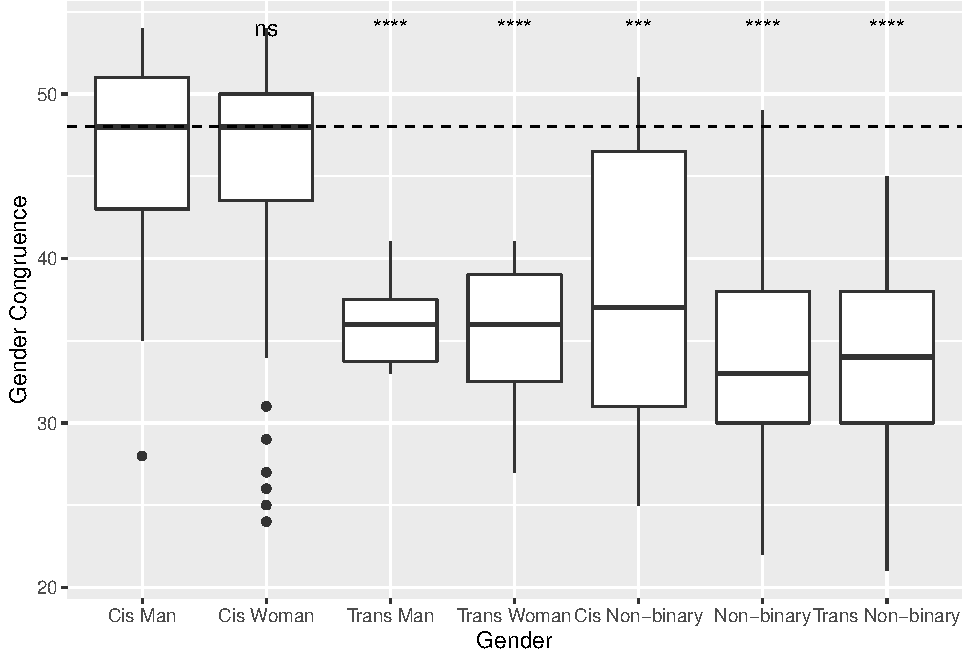
\includegraphics{thesis_files/figure-latex/unnamed-chunk-5-1.pdf}
\caption{\label{fig:unnamed-chunk-5}TCS Scores by Gender}
\end{figure}
A possible correlation between congruence and misgendering frequency was explored. A factorial ANOVA revealed that correlation had a significant effect on misgendering frequency, \emph{F}(1, 424) = 136.56, \emph{p} \textless{} 0.001 and felt stigma when misgendered, \emph{F}(1, 424) = 69.06, \emph{p} \textless{} 0.001, but not frequency and stigma together, \emph{F}(1, 424) = 0.2, \emph{p} = 0.65.

\hypertarget{transgender-inclusive-behaviors}{%
\section{Transgender Inclusive Behaviors}\label{transgender-inclusive-behaviors}}

Kattari, O'Connor, \& Kattari (2018) developed the Transgender Inclusive Behavior Scale (TIBS) as a method of quantifying the number of behaviors that may support and include transgender people that one regularly does. Scores are a sum of responses on a series of five-point likert scales ranging from ``Never'' to ``Often.''

A single-sample t-test revealed that non-cisgender people (\emph{M} = 51.34, \emph{SD} = 9.14) reporting performing more inclusive behaviors than cisgender people (\emph{M} = 41.98, \emph{SD} = 9.26), \emph{t}(304.22) = 10.22, \emph{p} \textless{} 0.001.

A one-way ANOVA demonstrated that there was a significant effect of gender \emph{F}(6, 260) = 26.14, \emph{p} \textless{} 0.001.
A Tukey post-hoc comparison revealed that cisgender men (\emph{M} = 37.31, \emph{SD} = 8.92) do significantly fewer trans inclusive behaviors than cisgender women (\emph{M} = 44.43, \emph{SD} = 8.18), transgender men (\emph{M} = 55.91, \emph{SD} = 9.16), transgender women (\emph{M} = 50.58, \emph{SD} = 9.97), cisgender non-binary people (\emph{M} = 45.73, \emph{SD} = 8.18), non-binary people (\emph{M} = 49.26, \emph{SD} = 9.3), and transgender non-binary people (\emph{M} = 53.85, \emph{SD} = 7.71). Cisgender women do significantly fewer trans inclusive behaviors than transgender men, transgender women, non-binary people, and transgender non-binary people. Cisgender non-binary people also do fewer trans inclusive behaviors than transgender non-binary people.
\begin{figure}
\centering
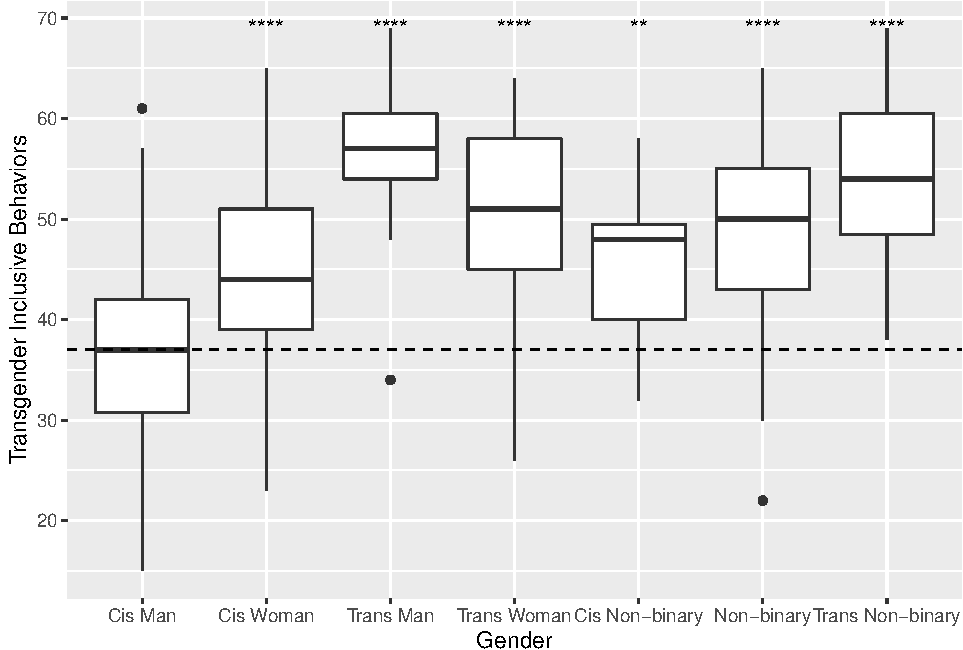
\includegraphics{thesis_files/figure-latex/unnamed-chunk-6-1.pdf}
\caption{\label{fig:unnamed-chunk-6}TIBS Scores by Gender}
\end{figure}
\hypertarget{pronouns-1}{%
\section{Pronouns}\label{pronouns-1}}

\hypertarget{comfort-sharing-pronouns}{%
\subsection{Comfort sharing pronouns}\label{comfort-sharing-pronouns}}

Items 1, 2, 3, 7, 8, and 9 touched on participant's comfort sharing their pronouns.
A one-way ANOVA found a significant effect of setting, gender, and pronouns on comfort sharing pronouns, \emph{F}(2, 1311) = 16.39, \emph{p} \textless{} 0.001. A post-hoc Tukey test found that generally, students are more comfortable sharing pronouns in class, (\emph{M} = 4.5, \emph{SD} = 0.98), and in non-academic settings at Reed, (\emph{M} = 4.43, \emph{SD} = 1.07), than they are in general, (\emph{M} = 4.14, \emph{SD} = 1.31). It also found that cisgender men, (\emph{M} = 4.65, \emph{SD} = 0.78), are more comfortable sharing their pronouns than trans men, (\emph{M} = 4.11, \emph{SD} = 1.24), trans women, (\emph{M} = 3.22, \emph{SD} = 1.51), and non-binary people, (\emph{M} = 3.66, \emph{SD} = 1.4).

One-way ANOVAs were used on each setting to elucidate effects of gender and pronoun within each setting. There were significant effects of gender in general, \emph{F}(6, 435) = 34.7, \emph{p} \textless{} 0.001, in non-academic settings at Reed, \emph{F}(6, 435) = 9.07, \emph{p} \textless{} 0.001, and in class, \emph{F}(6, 435) = 19.93, \emph{p} \textless{} 0.001. There were also significant effects of pronouns in general, \emph{F}(435, 435) = NA, \emph{p} = NA, in non-academic settings at Reed, \emph{F}(435, 435) = NA, \emph{p} = NA, and in class, \emph{F}(435, 435) = NA, \emph{p} = NA.

Post-hoc Tukey tests were used to compare gender groups within each setting. In a general setting, cis men, (\emph{M} = 4.53, \emph{SD} = 0.93), were more comfortable sharing their pronouns than trans women, (\emph{M} = 4.76, \emph{SD} = 0.68), non-binary people, (\emph{M} = 3.02, \emph{SD} = 1.5), and transgender non-binary people, (\emph{M} = 3.25, \emph{SD} = 1.49). In addition, cis women, (\emph{M} = 4.76, \emph{SD} = 0.68) were more comfortable sharing their pronouns than trans men, (\emph{M} = 3.67, \emph{SD} = 1.67), trans women, cisgender non-binary people, (\emph{M} = 3.87, \emph{SD} = 1.13), non-binary people, and transgender non-binary people. In non-academic settings at Reed, cis men, (\emph{M} = 4.59, \emph{SD} = 0.85), and cis women, (\emph{M} = 4.59, \emph{SD} = 0.85), were more comfortable sharing their pronouns than trans women, (\emph{M} = 3.4, \emph{SD} = 1.6), cis non-binary people, (\emph{M} = 3.8, \emph{SD} = 1.52), non-binary people, (\emph{M} = 4.04, \emph{SD} = 1.16), and trans non-binary people, (\emph{M} = 4.1, \emph{SD} = 1.39). In class, cis men, (\emph{M} = NA, \emph{SD} = NA), and cis women, (\emph{M} = 4.85, \emph{SD} = 0.53), were more comfortable sharing their pronouns than trans women, (\emph{M} = 3.35, \emph{SD} = 1.57), non-binary people, (\emph{M} = NA, \emph{SD} = NA), and trans non-binary people, (\emph{M} = 4.17, \emph{SD} = 1.14). Cis women were also more comfortable sharing their pronouns than cis non-binary people, (\emph{M} = 4.4, \emph{SD} = 0.83). Finally, trans women were less comfortable sharing their pronouns than cis non-binary people and trans non-binary people.

A one-way ANOVA was used to examine effects of social factors, gender, and pronouns on comfort sharing pronouns. Specifically, we examined whether people were more comfortable sharing their pronouns when a professor did so first, when someone else did first, and when the participant was with people of similar genders to their own. There were significant effects of social factor, \emph{F}(2, 1311) = 60.03, \emph{p} \textless{} 0.001, gender, \emph{F}(6, 1311) = 6.95, \emph{p} \textless{} 0.001, and pronouns, \emph{F}(6, 1311) = 15.66, \emph{p} \textless{} 0.001. A post-hoc Tukey test revealed that someone else saying their pronouns first makes the largest difference in making others comfortable sharing their pronouns. This is followed by the professor sharing their pronouns first, and finally the presence of people of similar genders to one's own.

\hypertarget{desire-to-share-pronouns}{%
\subsection{Desire to share pronouns}\label{desire-to-share-pronouns}}

Items 4, 5, and 6 touched on participant's desire to share their pronouns. A one-way ANOVA revealed significant effects of setting, \emph{F}(2, 1314) = 18.12, \emph{p} \textless{} 0.001, gender, \emph{F}(6, 1314) = 7.22, \emph{p} \textless{} 0.001, and pronouns \emph{F}(6, 1314) = 13.46, \emph{p} \textless{} 0.001. A post-hoc Tukey test revealed that people;s desire to share their pronouns is highest in classroom settings, followed by non-accade mic ettings atReed, and then lowest in general. Trans men reported a higher desire to share their pronouns than cisgender men, cisgender women, transgender women, cisgender non-binary people, and non-binary people. Transgender non-binary people also reported a higher desire to share their pronouns than cisgender men and non-binary people.

\hypertarget{concerns-about-sharing-pronouns}{%
\subsection{Concerns about sharing pronouns}\label{concerns-about-sharing-pronouns}}

Items 10, 11, and 12 touched on participant's concern that sharing their pronouns would draw unwanted attention to themselves. There were significant effects of setting, \emph{F}(2, 1314) = 27.49, \emph{p} \textless{} 0.001, gender \emph{F}(6, 1314) = 19.69, \emph{p} \textless{} 0.001, and pronouns, \emph{F}(6, 1314) = 23.44, \emph{p} \textless{} 0.001 on concern that sharing one's pronouns would draw unwanted attention to oneself. A post-hoc Tukey test revealed that participants were most concerned that sharing their pronouns would draw unwanted attention to them in general, followed by in non-academic settings at Reed, and least concerned in class.

\hypertarget{congruence-and-perception-of-pronouns}{%
\subsection{Congruence and perception of pronouns}\label{congruence-and-perception-of-pronouns}}

Items 13, 14, 15, 16, 17 and 18 touched upon participant's relationship to their pronouns, gender, and appearance. We ran one-way ANOVAs examing effects of gender and pronouns on each item with pos-hoc Tukey tests where relevant.

On item 13 (``I feel that the gender that people perceive me as and my pronouns are consistent with one another.''), there was a significant effect of gender, \emph{F}(6, 449) = 116.89, \emph{p} \textless{} 0.001. A post-hoc Tukey test found that cis men, (\emph{M} = 4.76, \emph{SD} = 0.6), experience higher consistency than trans men, (\emph{M} = 2.58, \emph{SD} = 1.62), trans women, (\emph{M} = 2.05, \emph{SD} = 1.1), cis non-binary people, (\emph{M} = 3.13, \emph{SD} = 1.77), non-binary people, (\emph{M} = 2.2, \emph{SD} = 1.27), and trans non-binary people, (\emph{M} = 1.85, \emph{SD} = 1.07). Cis women, (\emph{M} = 4.65, \emph{SD} = 0.85), also experience higher consistency than trans men, trans women, cis non-binary people, non-binary people, and trans non-binary people. Cis non-binary people also experience higher consistency than trans women. Finally, cis non-binary people experience higher consistency than non-binary people and trans non-binary people. There were no other significant differences between groups.

On item 14 (``I feel that my internal gender identity and pronouns are consistent with one another.''), there was a significant effect of gender, \emph{F}(6, 430) = 18.52, \emph{p} \textless{} 0.001 and pronouns, \emph{F}(6, 430) = 3.87, \emph{p} \textless{} 0.001. A post-hoc Tukey test found that cis men, (\emph{M} = 4.59, \emph{SD} = 0.8), and cis women, (\emph{M} = 4.53, \emph{SD} = 0.93), reported higher consistency than cis non-binary people, (\emph{M} = 3.07, \emph{SD} = 1.67), non-binary people, (\emph{M} = 3.23, \emph{SD} = 1.42), and trans non-binary people, (\emph{M} = 3.85, \emph{SD} = 1.34). Trans men, (\emph{M} = 4.5, \emph{SD} = 1.17), also reported higher consistency than cis non-binary people and non-binary people. Trans non-binary people also reported higher consistency than non-binary people. People who use they/them and she/her pronouns, (\emph{M} = 3.03, \emph{SD} = 1.53), reported higher consistency than people who just used they/them pronouns, (\emph{M} = 3.85, \emph{SD} = 1.21). There were no other significant differences between groups.

On item 15 (``I feel that my pronouns represent my gender identity well.''), there was a significant effect of gender, \emph{F}(6, 450) = 14.67, \emph{p} \textless{} 0.001. A post-hoc Tukey test revealed that cis men, (\emph{M} = 4.35, \emph{SD} = 1.06), and cis women, (\emph{M} = 4.39, \emph{SD} = 1.07), reported higher representativeness than cis non-binary people, (\emph{M} = 3.07, \emph{SD} = 1.67), non-binary people, (\emph{M} = 3.11, \emph{SD} = 1.46), and trans non-binary people, (\emph{M} = 3.71, \emph{SD} = 1.3). Furthermore, trans men, (\emph{M} = 4.5, \emph{SD} = 0.9), reported higher representativeness than cis non-binary people and non-binary people. There were no other significant differences between groups.

On item 16 (``If I don't tell people what my pronouns are, they will misgender me.''), there was a significant effect of gender, \emph{F}(6, 450) = 75.91, \emph{p} \textless{} 0.001. A post-hoc Tukey test revealed that cis men, (\emph{M} = 1.95, \emph{SD} = 0.3), and cis women, (\emph{M} = 1.91, \emph{SD} = 0.47), are misgendered significantly less when they do not share their pronouns when compared to trans men, (\emph{M} = 3.75, \emph{SD} = 1.54), trans women, (\emph{M} = 4.1, \emph{SD} = 1.25), non-binary people, (\emph{M} = 3.32, \emph{SD} = 1.54), and trans non-binary people, (\emph{M} = 4.31, \emph{SD} = 1.17). Furthermore, cis non-binary, (\emph{M} = 2.47, \emph{SD} = 0.92), people are misgendered significantly less than trans men, trans women, and non-binary people. There were no other significant differences between groups.

On item 17 (``I don't need to tell people what my pronouns are, because they usually assume correctly.''), there was a significant effect of gender, \emph{F}(6, 449) = 78.45, \emph{p} \textless{} 0.001. A post-hoc Tukey test revealed that people correctly assume cis men's, (\emph{M} = 4.56, \emph{SD} = 0.95), and cis women's, (\emph{M} = 4.49, \emph{SD} = 1.09), pronouns more frequently when compared to trans men, (\emph{M} = 2.5, \emph{SD} = 1.17), trans women, (\emph{M} = 2.15, \emph{SD} = 1.04), cis non-binary people, (\emph{M} = 3.27, \emph{SD} = 1.58), non-binary people, (\emph{M} = 2.46, \emph{SD} = 1.2), and trans non-binary people, (\emph{M} = 1.92, \emph{SD} = 0.65). Cis non-binary people's pronouns are also assumed correctly more frequently than trans women's and trans non-binary people.

Finally, on item 18 (``I feel like people understand me better when I share my pronouns.''), there was a significant effect of gender, \emph{F}(6, 449) = 25.69, \emph{p} \textless{} 0.001. A post-hoc Tukey test revealed that trans men, (\emph{M} = 3.58, \emph{SD} = 1.56), trans women, (\emph{M} = 3.7, \emph{SD} = 1.22), non-binary people, (\emph{M} = 3.67, \emph{SD} = 1.22), and trans non-binary, (\emph{M} = 3.98, \emph{SD} = 1.12), people feel better understood when they share their pronouns when compared to cis men, (\emph{M} = 2.39, \emph{SD} = 0.93) and cis women, (\emph{M} = 2.54, \emph{SD} = 0.96).

\hypertarget{historical-experience-at-reed-college}{%
\subsection{Historical experience at Reed College}\label{historical-experience-at-reed-college}}

Item 19 (``In classes at Reed, professors usually introduce themselves with their pronouns'') asked students to report how frequently professors introduced themselves with their pronouns. A one-way ANOVA did not find a significant effect of gender, \emph{F}(6, 339) = 1.97, \emph{p} = 0.07, or major, \emph{F}(70, 339) = 1.26, \emph{p} = 0.1, on reported frequency of professors sharing their pronouns. However, when we only compared majors in which we had more than 5 students in, there were significant effects of both gender, \emph{F}(6, 311) = 2.12, \emph{p} = 0.05, and major, \emph{F}(20, 311) = 2.17, \emph{p} \textless{} 0.001.

Item 20 (``In classes at Reed, students usually introduce themselves with their pronouns'') asked students to report how often their peers introduced themselves with their pronouns. A one-way ANOVA revaled a significant effect of gender, \emph{F}(6, 339) = 3.67, \emph{p} \textless{} 0.001, but not major. When we only compared majors that we had more than 5 students in, there were significant effects of gender, \emph{F}(6, 311) = 2.12, \emph{p} = 0.05, and major, \emph{F}(20, 311) = 2.17, \emph{p} \textless{} 0.001.

\hypertarget{primary-component-analysis}{%
\subsection{Primary Component Analysis}\label{primary-component-analysis}}

Principal component analysis (PCA) was used on the pronoun and misgendering data. Using a Screen plot, we retained three components with an eigenvalue of 2.99, accounting for 52.1\% of the variance.
\begin{longtable}{lrrr}
\toprule
Item & Comp. 1 & Comp. 2 & Comp. 3\\
\midrule
cis & -0.12 & -0.01 & 0.01\\
trans & 0.07 & 0.02 & 0.03\\
nonbinary & 0.11 & 0.01 & -0.02\\
gender.man & -0.04 & -0.03 & 0.03\\
gender.woman & -0.05 & 0.02 & 0.00\\
\addlinespace
comfort\_general & -0.25 & 0.23 & 0.09\\
comfort\_reed & -0.11 & 0.23 & 0.00\\
comfort\_class & -0.15 & 0.22 & 0.04\\
desire\_general & 0.01 & 0.41 & 0.04\\
desire\_reed & 0.11 & 0.41 & -0.03\\
\addlinespace
desire\_class & 0.06 & 0.41 & -0.03\\
comfort\_withsimilargenders & 0.27 & 0.21 & -0.03\\
comfort\_someoneelsefirst & 0.03 & 0.17 & 0.21\\
comfort\_proffirst & 0.03 & 0.19 & 0.20\\
attention\_general & 0.27 & -0.15 & 0.39\\
\addlinespace
attention\_reed & 0.11 & -0.18 & 0.56\\
attention\_class & 0.16 & -0.14 & 0.38\\
gender\_perception\_consistent & -0.40 & 0.02 & 0.26\\
gender\_pronouns\_consistent & -0.15 & 0.21 & 0.25\\
pronouns\_represent & -0.14 & 0.22 & 0.27\\
\addlinespace
willmisgender\_ifnopronouns & 0.30 & 0.08 & -0.06\\
assume\_pronouns\_correctly & -0.37 & -0.02 & 0.13\\
understand\_better & 0.20 & 0.19 & 0.02\\
profs\_share & -0.09 & 0.01 & -0.17\\
students\_share & -0.04 & 0.03 & -0.06\\
\addlinespace
reed\_support & -0.19 & -0.09 & -0.06\\
misgendering\_freq & 0.30 & 0.02 & -0.08\\
misgendering\_stigma & 0.24 & 0.12 & 0.15\\
\bottomrule
\end{longtable}
Inspection of the first component's loadings indicate that concern that consistency between others' perception of one's gender, others' assumptions about gender and pronouns, misgendering, and comfort when with people with similar genders to one's own are making significant contributions to the first component. Because these items are mainly concerned with the assumptions other people place on one's gender and pronouns, this component appears to be the amount that cisnormative assumptions about one's gender and appearance harms individuals.

Loadings from the second component encompasses one's desire to share one's pronouns in various settings, as well as how comfortable one feels doing so. Because the largest loading in the second component is one's desire to share pronouns, this seems to indicate one's readiness to share pronouns.

Loadings from the third component emphasize concern that sharing one's pronouns will draw unwanted attention, as well as when others---not necessarily of the same gender---share their pronouns first and how consistent and representative one's pronouns are with one's gender. This component appears to represent concern around sharing pronouns and fears of judgment or lack of understanding about one's pronouns.
\begin{figure}
\centering
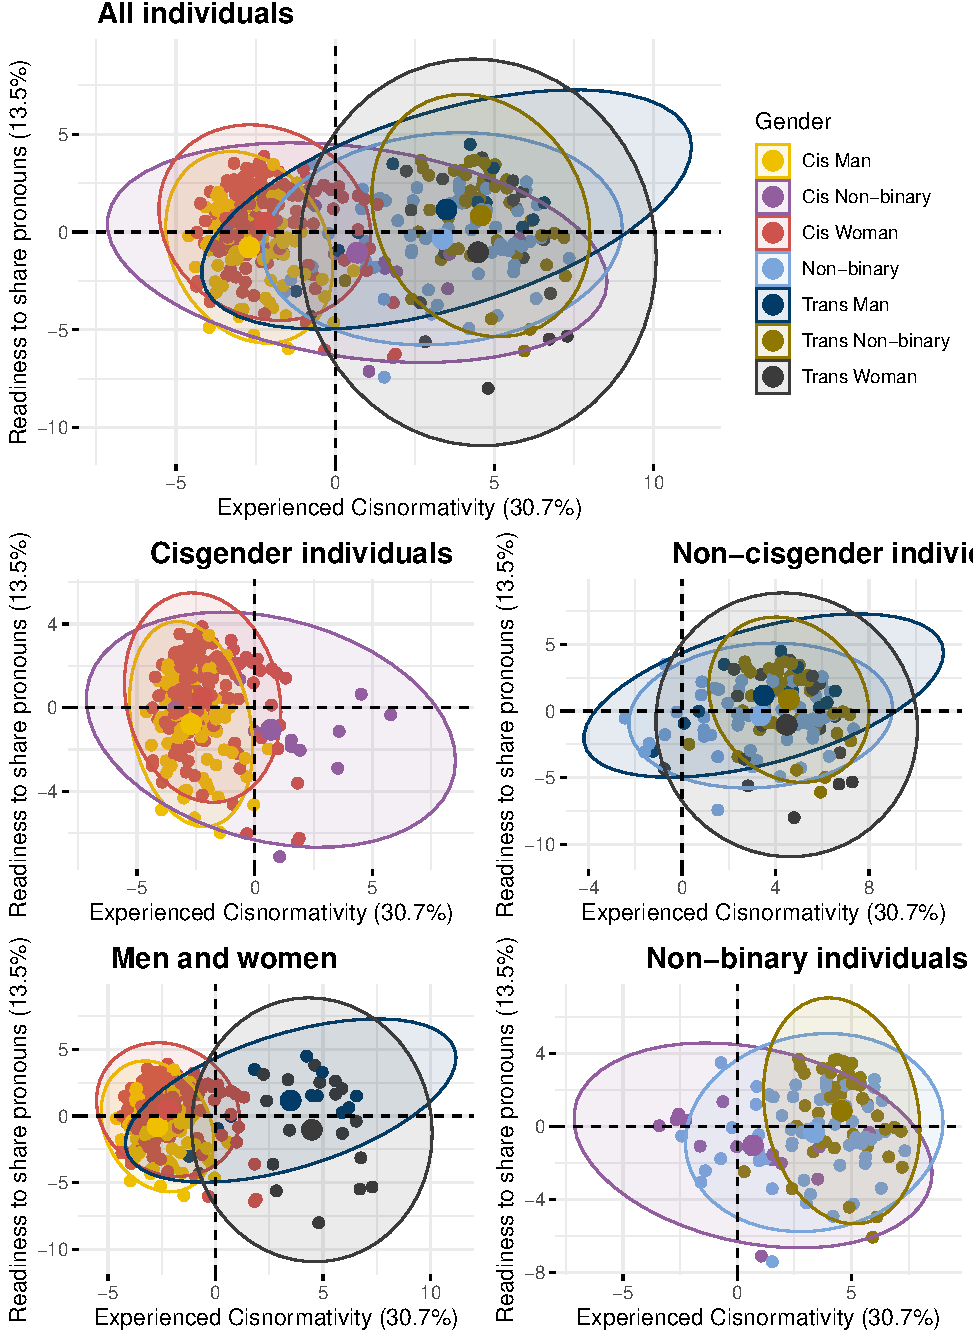
\includegraphics{thesis_files/figure-latex/pca_comp_1_2-1.pdf}
\caption{(\#fig:pca\_comp\_1\_2)PCA Components 1 \& 2 by Gender}
\end{figure}
A one-way ANOVA demonstrated a significant effect of gender on the first component, \emph{F}(6, 391) = 226.3, \emph{p} \textless{} 0.001. A post-hoc Tukey test revealed that cisgender men, (\emph{M} = -2.72, \emph{SD} = 1.09), and women, (\emph{M} = -2.25, \emph{SD} = 1.37), are significantly less affected by cisnormativity than trans men, (\emph{M} = 3.28, \emph{SD} = 2.62), trans women, (\emph{M} = 4.32, \emph{SD} = 2), cisgender non-binary people, (\emph{M} = 0.64, \emph{SD} = 2.87), non-binary people, (\emph{M} = 3.4, \emph{SD} = 2.22), and transgender non-binary people, (\emph{M} = 4.56, \emph{SD} = 1.35). Cisgender non-binary people are also less affected than trans men, trans women, non-binary people, and transgender non-binary people. Trans non-binary people are also more affected than non-binary people.
\begin{figure}
\centering
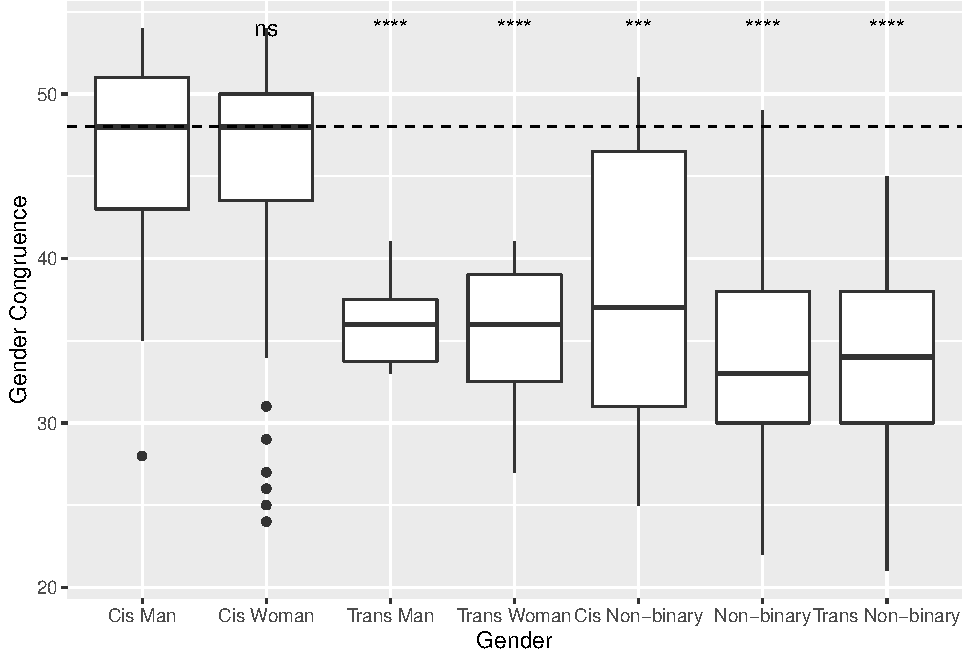
\includegraphics{thesis_files/figure-latex/unnamed-chunk-7-1.pdf}
\caption{\label{fig:unnamed-chunk-7}PCA Component 1 by Gender}
\end{figure}
Visualization of the first component indicated possible bimodality along the first component. Hartigan's dip test indicated that the distribution along the first component is unlikely to be unimodal, (\emph{D} = 0.032, \emph{p} = 0.006). This indicates that experiences with cisnormativity may be as bimodal. This indicates that cisgender and non-cisgender people may have significantly different experiences navigating the world as their gender.

Another one-way ANOVA demonstrated a significant effect of gender on the second component, \emph{F}(6, 391) = 6.15, \emph{p} \textless{} 0.001. A post-hoc Tukey test revealed that cisgender men, (\emph{M} = -2.72, \emph{SD} = 1.09), are less willing to share their pronouns than cisgender women, (\emph{M} = -2.25, \emph{SD} = 1.37) trans men, (\emph{M} = 3.28, \emph{SD} = 2.62), and non-binary people, (\emph{M} = 3.4, \emph{SD} = 2.22). Non-binary people are also more willing to share their pronouns than transgender women, (\emph{M} = 4.32, \emph{SD} = 2).
\begin{figure}
\centering
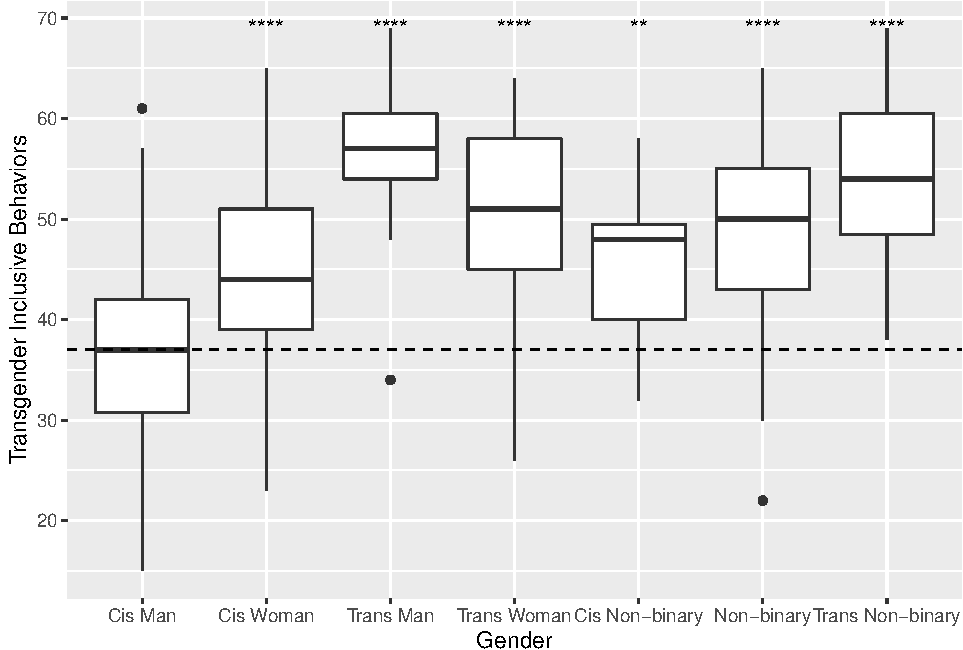
\includegraphics{thesis_files/figure-latex/unnamed-chunk-8-1.pdf}
\caption{\label{fig:unnamed-chunk-8}PCA Components 1 \& 3 by Gender}
\end{figure}
A final one-way ANOVA demonstrated a significant effect of gender on the third component, \emph{F}(6, 391) = 4.27, \emph{p} \textless{} 0.001. Non-binary people, (\emph{M} = 3.4, \emph{SD} = 2.22), are significantly less concerned that sharing their pronouns will draw unwanted attention than cisgender men, (\emph{M} = -2.72, \emph{SD} = 1.09), cisgender women, (\emph{M} = -2.25, \emph{SD} = 1.37), transgender men (\emph{M} = 3.28, \emph{SD} = 2.62), and transgender women (\emph{M} = 4.32, \emph{SD} = 2). There were no significant effects between any other groups.

However, this may be due to the fact that this is the third component which only accounts for 7.8\% of the total variation. Visualization of the third component shows that there is considerable variation within groups.

\hypertarget{discussion}{%
\chapter{Discussion}\label{discussion}}

Placeholder

\hypertarget{gender-identity}{%
\section{Gender Identity}\label{gender-identity}}

\hypertarget{pronouns-2}{%
\section{Pronouns}\label{pronouns-2}}

\hypertarget{experiences-with-misgendering-1}{%
\section{Experiences with Misgendering}\label{experiences-with-misgendering-1}}

\hypertarget{gender-congruence-1}{%
\section{Gender Congruence}\label{gender-congruence-1}}

\hypertarget{transgender-inclusive-behaviors-1}{%
\section{Transgender Inclusive Behaviors}\label{transgender-inclusive-behaviors-1}}

\hypertarget{primary-component-analysis-1}{%
\section{Primary Component Analysis}\label{primary-component-analysis-1}}

\hypertarget{limitations}{%
\section{Limitations}\label{limitations}}

\appendix

\hypertarget{appendix}{%
\chapter*{Appendix}\label{appendix}}
\addcontentsline{toc}{chapter}{Appendix}

\hypertarget{references}{%
\chapter*{References}\label{references}}
\addcontentsline{toc}{chapter}{References}

Placeholder

\hypertarget{refs}{}
\begin{cslreferences}
\leavevmode\hypertarget{ref-kattariDevelopmentValidationTransgender2018}{}%
Kattari, S. K., O'Connor, A. A., \& Kattari, L. (2018). Development and Validation of the Transgender Inclusive Behavior Scale (TIBS). \emph{Journal of Homosexuality}, \emph{65}(2), 181--196. \url{http://doi.org/10.1080/00918369.2017.1314160}

\leavevmode\hypertarget{ref-kozeeMeasuringTransgenderIndividuals2012}{}%
Kozee, H. B., Tylka, T. L., \& Bauerband, L. A. (2012). Measuring Transgender Individuals' Comfort With Gender Identity and Appearance: Development and Validation of the Transgender Congruence Scale. \emph{Psychology of Women Quarterly}, \emph{36}(2), 179--196. \url{http://doi.org/10.1177/0361684312442161}

\leavevmode\hypertarget{ref-mclemoreExperiencesMisgenderingIdentity2015}{}%
McLemore, K. A. (2015). Experiences with Misgendering: Identity Misclassification of Transgender Spectrum Individuals. \emph{Self and Identity}, \emph{14}(1), 51--74. \url{http://doi.org/10.1080/15298868.2014.950691}

\leavevmode\hypertarget{ref-reedcollegeinstitutionalresearchFactsReed2019}{}%
Reed College Institutional Research. (2019). Facts about Reed. Retrieved April 27, 2020, from \url{https://www.reed.edu/ir/enrollment.html}
\end{cslreferences}

% Index?

\end{document}
